\chapter{Аналитический раздел}
\label{cha:analysis}
\section{Цель и задачи работы}
Целью данной работы является создание программного комплекста для обнаружения выбросов временных рядов в собираемых данных.
Для достижения данной цели необходимо решить следующие задачи:
\begin{itemize}
	\item ПЕРЕПИСАТЬ ИЗ ПРЕЗЕНТАЦИИ
	\item пронализировать предметную область и существующие методы обнаружения выбросов
	\item разработать метод обнаружения выбросов
	\item smth
	\item создать ПО, реализующего  разработанный метод обнаружения выбросов
	\item провести вычислительный эксперименты с использованием разработанного метода
	
\end{itemize}
\section{Обнаружение аномалий}
В машинном обучении обнаружение  "ненормальных" экземпляров в наборах данных всегда представляло большой интерес. Этот процесс широко известен как обнаружение аномалий или обнаружение выбросов.  Вероятно, первое определение было дано Граббсом\cite{Book02} в 1969 году: "Относительное наблюдение или выброс - это элемент выборки, который, заметно отличается от других членов выборки, в которых он встречается ".
Хотя это определение по-прежнему актуально и сегодня, мотивация для обнаружения этих выбросов сейчас совсем другая. Тогда основная причина обнаружения заключалась в том, чтобы удалить выбросы из данных для обучения, поскольку алгоритмы распознавания  были весьма чувствительны к выбросам в данных. Эта процедура также называется очищением данных. После разработки более надежных классификаторов интерес к обнаружению аномалий значительно снизился. Однако в 2000 году произошел поворотный момент, когда исследователи стали больше интересоваться самими аномалиями, поскольку они часто связаны с особенно интересными событиями или подозрительными данными. С тех пор было разработано много новых алгоритмов, которые оцениваются в этой статье. В этом контексте определение Граббса также было расширено, так что сегодня аномалии, как известно, имеют две важные характеристики:
\begin{enumerate}
	\item Аномалия отличается от нормы по своим особенностям
	\item Аномалия редко встречается в наборе данных по сравнению с "нормальными" данными
\end{enumerate}
\subsection{Классификация методов обнаружений аномалий}
В отличие от хорошо известной  системы классификации, где учебные данные используются для обучения классификатора, а результаты измерений данных оцениваются впоследствии, возможно множество вариантов, когда речь идет об обнаружении аномалий. Метод обнаружения аномалий, которая будет использоваться, зависит от ярлыков, доступных в наборе данных, и мы можем выделить три основных типа:
\begin{enumerate}
\item Обучение с учителем. Доступны полностью размеченные данные для обучения и для тестов. Обычный классификатор может быть обучен один раз и применяться впоследствии. Это похоже на традиционное распозвание образов, за исключением того, что классы обычно сильно не сбалансированы. Поэтому не все алгоритмы классификации идеально подходят для этой задачи. Для многих применений аномалии не известны заранее или могут возникать спонтанно в качестве новинок на этапе тестирования.
\item Обучение с частичным привлечением учителя.Обучение использует учебные и тестовые наборы данных. Данные обучения состоят только из нормальных данных без каких-либо аномалий. Основная идея заключается в том, что модель нормального класса изучается, а аномалии могут быть обнаружены впоследствии, отклоняясь от этой модели. Эта идея также известна как «одноклассовая» классификация \cite{Book03}.
\item Обучение без учителя.
Самый гибкий способ, который не требует каких-либо меток. Кроме того, нет различия между учебным и тестовым наборами данных. Идея заключается в том, что алгоритм обнаружения аномалии оценивает данные исключительно на основе внутренних свойств набора данных. Как правило, расстояния или плотности используются для оценки того, что является нормальным, а что является выбросом. В этой работе основное внимание будет этому  именно этому способу. Так же этот способ иногда называют "неконтролируемый способ обнаружения  аномалий".
\end{enumerate}
\subsection{Признакое представление данных}
В дальнейшем будем исходить из предположения что  данные имеют признаковое представление, т.е. каждый объект х  представлен в виде вектора $\mathbb{R}^d$. В задаче обучения без учителя задача обнаружения аномалий  формулируется следующим образом: в заданном множестве X для каждого элемента выдать 0, если этот объект относится. При этом правильных ответов не предоставляется.

В аналогиченой задаче обучения с учителем на некоторой выборке входных данных $X_train$, называемой тренировочной выборкой, известен правильный ответ, т.е для каждого элемента $x \in X_train$ представлены метки $ y \in {0,1} $, характирующие является ли объект аномалией или нет. Для выборки данных, для которой метки не предоставлены, задача сводится к задаче бинарной классификации, а значит может решаться при помощи любых алгоритмов  машиного обучения с учителем. Возможны и "вырожденные" случаи, когда все метки тренировочного набора данных одинаковы. В таком случае алгоритмы выдают неправильный результат.

к классу нормальных данных, и 1, если этот объект аномален.
\section{Результат метода обнаружения аномалий}
Существует два варианта выходных данных алгоритма обнаружения аномалии. Во-первых, метка может использоваться как результат, указывающий, является ли экземпляр аномалией или нет. Во-вторых, оценка или достоверность могут быть более информативным результатом, указывающим на степень аномалии. А алгоритмах метода обучения с учителем зачастую используются метки как выходные данные. С другой стороны, для алгоритмах  с частичным привлечением учителя и без учителя  обнаружения аномалий чаще встречаются оценки.
\section{Виды аномалий}
\begin{figure}
	\centering
	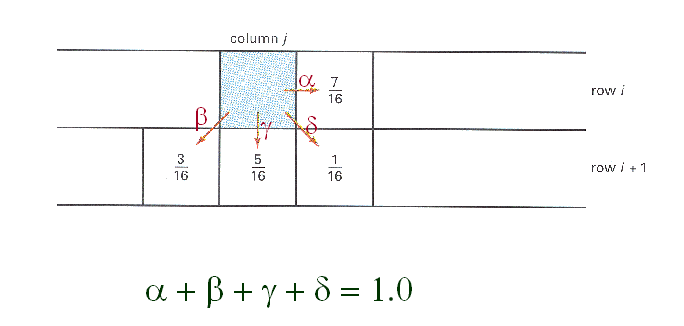
\includegraphics[width=.5\textwidth]{img/1.png}
	\caption{Простой двумерный пример}
	\label{fig01}
\end{figure}

Основная идея алгоритмов обнаружения аномалий заключается в обнаружении экземпляров данных в наборе данных, которые отклоняются от нормы. Однако на практике существует множество случаев, когда это основное предположение является неоднозначным. На рис. 2 показаны некоторые из этих случаев с использованием простого двумерного набора данных. Две аномалии могут быть легко идентифицированы визуально: красные точки  сильно отличаются отличаются значениям параметров от областей плотной группировки точек  и поэтому называются глобальными аномалиями.Когда мы смотрим на весь набор данных в целом, то фиолетовую точку можно отнести к тому же классу, что и зеленые тчки.  Однако, когда мы фокусируемся только на кластере зеленых точек и сравниваем его с фиолетовой, пренебрегая всеми другими точками, то её можно рассматривать как аномалию. Поэтому фиолетовая точка называется локальной аномалией, так как она аномальна по сравнению с ее близкой окрестностью. В зависимости от цели исследования,нас могут интересовать   местные аномалии или нет. Другой интересный вопрос заключается в том, следует ли рассматривать точки черного кластера  как три аномалии или как (небольшой) кластер. Эти явления называются микрокластерами, а алгоритмы обнаружения аномалий должны присваиваеть  оценку(вероятность того, что точка является аномалией)ему точкам этого кластера значения большие, чем точкам зеленого кластера, но меньше, чем красным точкам. Этот простой пример уже показывает, что аномалии не всегда очевидны, а оценка намного полезнее, чем назначение двоичных меток.

Обычно под аномалией принимают точки красные точки, так как их характеристики значельно отличаются от характеристик датасета, а так же их небольшое количество.Однако, такой принцип обнаружения иногда терпит неудачу. Например, при хакерских ddos-атаках, большая часть трафика - необычная, аномальная. В этом случае алгоритм обучения без учителя потерпит неудачу и не сможет выделить хакерскую атака как аномальное поведение.

Задача обнаружения одиночных аномальных экземпляров в более крупном наборе данных (как это представлено до сих пор) называется обнаружением точечной аномалии\cite{Book04}. Сегодня почти все доступные неконтролируемые алгоритмы обнаружения  относятся к этому типу. Если аномальная ситуация представлена ​​как множество многих случаев, это называется коллективной аномалией. Каждый из этих экземпляров не обязательно является точечной аномалией, но только определенная их комбинация определяет аномалию. Предыдущим приведенным примером возникновения нескольких специфических шаблонов доступа при обнаружении ddos-атак является такая коллективная аномалия. Третий вид - это контекстуальные аномалии, которые описывают эффект, что точка может рассматриваться как нормальная, но когда данный контекст учитывается,то точка оказывается аномалией. Самым распространенным контекстом является время. В качестве примера предположим, что мы измеряем температуру в диапазоне от $-30^{\circ}$C до $+40^{\circ}$C в течение года. Таким образом, температура $25^{\circ}$C кажется довольно нормальной, но когда мы учитываем контекстное время (например, месяц), такая высокая температура $25^{\circ}$C  в течение зимы  будет рассматриваться как аномалия.

Алгоритмы обнаружения точечных аномалий так же можно использовать для обнаружения контекстуальных и коллективных аномалий. Для этого нужно включить сам контекст как параметр. В вышеприведенным примере включение месяца как дополнительного параметра поможет обнаружить аномалию. Однако в более сложных сценариях может потребоваться одна или несколько новых парметров, чтобы преобразовать задачу определения контекстной аномалии в проблему обнаружения точечной аномалии. Преобразование поиска коллективной аномалии в поиск одиночную может быть нетривиальной. Корреляция, агрегация и группировка используются  для создания нового набора данных с другим представлением признаков\cite{Book05} . Преобразование из задачи обнаружени коллективной аномалии в задачу обнаружения точечной аномалии требует глубоких знаний о наборе исходных данных и часто приводит  к существенным искажениям при переводе данных в новый формат. Такое семантическое преобразование называется  генерированием представления данных(\textit{англ. data view generation}).
  
  Таким образом можно сделать вывод, что многие задачи обнаружения аномалий требуют предварительной обработки данных перед передачей их на вход алгоритму. В противном случае можно получить формально верные, но фактические бесполезные результаты.
\subsection{Нормализация данных} 
Когда мы получили предварительно обработанный  датасет для поиска точечной аномалии, то последним шагом перед передачей в алгоритм, является нормализация данных. Нормализация данных предназначена для усранения зависимости от выбора единицы измерения и заключается в преобразовании диапазонов значений всех атрибутов к стандартным интервалам([0,1] или [-1,1])\cite{Book06}. Нормализация данных направлена на придание всем атрибутам одинакового "веса".
\subsubsection{Основные методы нормализация данных}
\begin{enumerate}
	\item Min-max нормализация заключается в применении к диапазону значений атрибута х линейного преобразования, которое отображает [min(х),max(х)] в [A,B].
	\begin{equation}
	x^\prime_i=\uptau(x_i)=\frac{x_i - min(x)}{max(x) - min(x)}*(B-A) + A
		\end{equation}
   \begin{equation}
		x \in[min(x), max(x)] \Rightarrow \uptau(х) \Rightarrow [A,B]
	\end{equation}
	Min-max нормализация сохраняет все зависимости и порядок оригинальных значений атрибута. Недостатком этгого метода является то, что выбросы могут сжать основную массу значений к очень маленькому интервалу
	\item Z-нормализация  основывается на приведении распределения исходного атрибута х  к центрированному распределению со стандартным отклоненим, равным 1 \cite{Book06} .
	\begin{equation}
	x^\prime_i=\uptau(x_i) =\frac{x_i - \overline{x}}{\sigma_x}
		\end{equation}
		\begin{equation}
		M[x^\prime]=1	 
		\end{equation}
		\begin{equation}
		D[\overline{x}^\prime]=0	 
		\end{equation}
		Метод полезен когда в данных содержат выбросы.
	\item Масштабирование заключается в изменении длины вектора значений атрибута путем умножения на константу \cite{Book06} .
	\begin{equation}
	x^\prime_i=\uptau(x_i)=\lambda*x_i
	\end{equation}
	Длина вектора х уменьшается при $|\lambda|<1$ и увеличивается при $|\lambda|>1$ 
\end{enumerate}
\section{Неконтролируемые алгоритмы обнаружения аномалий}
\subsection{Вероятностный подход}
Основная идея генеративного подхода заключается в использование вероятноского смесевого моделирования данных. Предлагается подобрать такую вероятностую модель, из которой было получены нормированные данные. Такие модели обычно называются генеративными моделями, где для каждой точки(элемента данных) можем посчитать генеративную вероятность(или вероятность правдоподобия).Т.е. задача  сводится к нахождению плотности распределения p(x). Аномиями при этом  считаются точки(элементы набора данных), имеющию низкое правдоподобие. В качестве показателя аномальности выступает функция p.

Для построения генеративной модели нужно решить следующую задачу:
	\begin{equation}
	\prod \limits_{x \in X_{norm}} p(x,\theta)  \rightarrow max_\theta
		\end{equation}
		где $ X_{norm}$ - нормальные данные представленного набора данных ${p(x,\theta)|\theta \in \omega}$ -семейство плотностей вероятностей, параметризованные $\theta$;
		
Этот метод редко используется на практике, так как тяжело проверить полученную генеративную модель на адекватность, сложно  убедится в правильном выборе семейства смесевых распределений. Это связано с тем, что низкое значение функции правдоподобия может означать как и аномальное значение, так и неудачно подобранную модель. Этот метод применяется с опорой на априорную информацию, в случае когда можно проверить полученную модель на адекватность.
\subsection{Линейный подход}
Основной идей линейного подхода является построение некой  модели, характеризующей нормальные данные. Точки, которые значительно отклоняются от этой модели, считаются аномалиями.

Предполагается, что нормальные данные  находятся в подпрострастрансве пространства атрибутов данных(размер подпространства атирбутов данных равен размерности данных). В свою очередь, задача линейного метода - найти низкоразмерное подпространства, такие что, выборка данных этого подпросранства значительно отличается от остальных точек пространства данных.

Одним из возможных вариантов решения является использование линейной регрессии. Выбирается одна из наблюдаемых переменных  набора данных и относительно неё решается задача линейной регрессии оставшихся атрибутов. Итоговым ответом будет является усредненное значения показателя аномалии по всем атрибутам. 

Алгоритмы, основанные на линейном подходе, требуют  наличия линейной зависимости атрибутов данных. 
\subsection{Метрические методы}
Метрические методы хорошо подоходят в случае когда данные не размечены. Сложность вычисления прямо как пропорциональна размерности данных m,как и их количеству n. При росте набора данных наблюдается экспоненциальный рост сложности вычислений. Однако, эти методы хорошо проявляют себя на ограниченных наборах данных\cite{Book7}. Следовательно такие методы как k-ближайших соседей(так же известный как обучение на основе примеров и описанный поздее) с нотацией ассимтпотического роста $O(n^2m)$ недопустимы для наборов данных с большой размерности, если их размерность не может быть уменьшена.

Существуют много  различных вариации алгоритма k-ближайших соседей для обнаружения аномалий, но все они основаны на вычислении некой метрики "расстояния до соседей", такой как Евклидово расстояние или  расстояние Махаланобиса. Евлидово расстояние задается следующей формулой:
 	\begin{equation}
 	\sqrt{\sum_{i=1}^n(x_i-y_i)^2}
 		\end{equation}
 и является просто расстоянием между двумя точка, когда как  расстояние Махаланобиса, задаваемое следующей формулой
 	\begin{equation}
 	\sqrt{(x-\mu)^T C^-1 (x-\mu)}
 	\end{equation}
 	вычисляет расстояние от точки до центра тяжести ($\mu$), определяемого формулой коррелированных атрибутов, заданных матрицей ковариации (C). Расстояние  Махаланобиса
 	рассчитывается значительно дольше по сравнению с евлидковым
 	 по сравнению с евклидовым расстоянием для для больших объемов данных, поскольку оно требует
 	пройти через весь набор данных, чтобы идентифицировать корреляции атрибутов.
 	
 Точка p является выбросом
если не более n - 1 других точек в наборе данных имеют более высокий $D_m$(расстояние до m соседей), где m задается. Например на рисунке 02\cite{fig02} черная точка является наиболее удаленной от соседей, следовательно она является выбросом. Красные точки расположены рядом друг с другом, однако расстояние до других точек велико, следовательно они тоже являются аномалиями. Такой подход воприимчив к вычислительному росту, потому что должна быть вычислена матрица расстояний точек друг от друга, поэтому Рамасвани в 2000 году предложил оптимизацию метода k-ближайших соседей(c англ. k-Nearest Neighbour - k-NN)  в виде составления ранжированного списка потенциальных выбросов.э

 Оптимизация Рамасвани заключается в разбиении данных на ячейки.Если какая-либо ячейка и ее ближайшие соседи содержат больше, чем k
 точек, то точки в ячейке считаются лежащими в плотной области
 поэтому содержащиеся точки вряд ли будут выбросами. Если же почти все ячейки содержат больше,чем k точек, а какие-то ячейки содержат меньше, чем k точек, то тогда все точки, лежащие в ячейках, которые содержат  менее k элементов, помечаются  аномальным. Следовательно,
 необходимо обработать только небольшое количество ячеек, которые ранее не были помечены и только относительно небольшое количество расстояний необходимовычислить для обнаружений аномалий
\begin{figure}
	\centering
	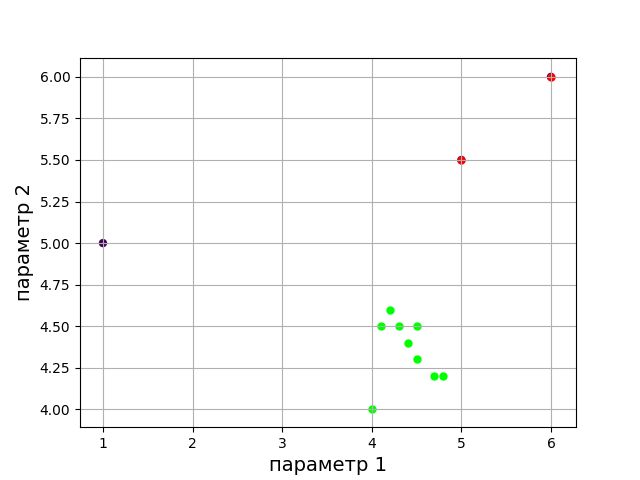
\includegraphics[width=.5\textwidth]{img/2.png}
	\caption{Пример k-ближайших соседей}
	\label{fig02}
\end{figure}
 


В анализе данных есть два основных направления, которорые занимаются поиском аномалий - это детектирование новизны и обнаружение выбросов. "Новый объект"- это так же объект, который отличается по своим свойствам от объектов  выборки. Однако, в отличие от выброса, он его ещё нет в самой выборке и задача анализа сводится к его обнаружению при появление. Например, если вы анализируете замеры уровня шума и отбрасываетете слишком высокие или слишком низкие значения, то вы боретесь с выбросам. А если Вы создаёте алгоритм, который для каждого нового замера оценивает, насколько он похож на прошлые, и выбрасывает аномальные — вы "боретесь с новизной"
\cite{Book01}.
Выбросы являются следствием:
\begin{enumerate}
	\item ошибок в данных
	\item неверно классифицированных объектов
	\item присутсвием объектов других выборок
	\item намеренным искажением данных
\end{enumerate}


На рисунке \ref{fig01} можно увидеть желтые точки - выброс "слабом смысле". Они незначительно отклоняются от основных данных(зеленые точки). Красные же точки являются аномальными - выбросами "в сильном смысле", они значительно  отклоняются с от основывных данных. В данной работе будет изучаться вопрос находждения "сильных выбросов" и  критериев отличия сильного выброса от основных данных. В дальнейшем под словом "выброс" будет подразумеваться "сильный выброс",  а под  аномалией - в выброс(выброс является частным случаем аномалии).
Понятие аномалии зачастую интерпетируют по-разному в зависимости от характера данных. Обычно аномалией назыют некоторое отклонение от нормы. Это определение нуждается в формальном уточнении.

\section{Постановка задачи}

% Обратите внимание, что включается не ../dia/..., а inc/dia/...
% В Makefile есть соответствующее правило для inc/dia/*.pdf, которое
% берет исходные файлы из ../dia в этом случае.

%\begin{figure}
%  \centering
%  \includegraphics[width=\textwidth]{inc/dia/rpz-idef0}
%  \caption{Рисунок}
%  \label{fig:fig01}
%\end{figure}

%\begin{figure}
%  \centering
%  \includegraphics[height=0.85\textheight]{inc/img/leonardo}
%  \caption{Предполагаемый автопортрет Леонардо да Винчи}
 % \label{fig:leonardo}
%\end{figure}

%В \cite{Pup09} указано, что...

Кстати, про картинки. Во-первых, для фигур следует использовать \texttt{[ht]}. Если и после этого картинки вставляются <<не по ГОСТ>>, т.е. слишком далеко от места ссылки, "--- значит у вас в РПЗ \textbf{слишком мало текста}! Хотя и ужасный параметр \texttt{!ht} у окружения \texttt{figure} тоже никто не отменял, только при его использовании документ получается страшный, как в ворде, поэтому просьба так не делать по возможности.

\section{Существующие подходы к созданию всячины}

Известны следующие подходы...

\begin{enumerate}
\item Перечисление с номерами.
\item Номера первого уровня. Да, ГОСТ требует именно так "--- сначала буквы, на втором уровне "--- цифры.
Чуть ниже будет вариант <<нормальной>> нумерации и советы по её изменению.
Да, мне так нравится: на первом уровне выравнивание элементов как у обычных абзацев. Проверим теперь вложенные списки.
\begin{enumerate}
\item Номера второго уровня.
\item Номера второго уровня. Проверяем на длииииной-предлиииииииииинной строке, что получается.... Сойдёт.
\end{enumerate}
\item По мнению Лукьяненко, человеческий мозг старается подвести любую проблему к выбору
  из трех вариантов.
\item Четвёртый (и последний) элемент списка.
\end{enumerate}

Теперь мы покажем, как изменить нумерацию на «нормальную», если вам этого захочется. Пара команд в начале документа поможет нам.

\renewcommand{\labelenumi}{\arabic{enumi})}
\renewcommand{\labelenumii}{\asbuk{enumii})}

\begin{enumerate}
\item Изменим нумерацию на более привычную...
\item ... нарушим этим гост.
\begin{enumerate}
\item Но, пожалуй, так лучше.
\end{enumerate}
\end{enumerate}

В заключение покажем произвольные маркеры в списках. Для них нужен пакет \textbf{enumerate}.
\begin{enumerate}[1.]
\item Маркер с арабской цифрой и с точкой.
\item Маркер с арабской цифрой и с точкой.
\begin{enumerate}[I.]
\item Римская цифра с точкой.
\item Римская цифра с точкой.
\end{enumerate}
\end{enumerate}

В отчётах могут быть и таблицы "--- см. табл.~\ref{tab:tabular} и~\ref{tab:longtable}.
Небольшая таблица делается при помощи \Code{tabular} внутри \Code{table} (последний
полностью аналогичен \Code{figure}, но добавляет другую подпись).

\begin{table}[ht]
  \caption{Пример короткой таблицы с коротким названием}
  \begin{tabular}{|r|c|c|c|l|}
  \hline
  Тело      & $F$ & $V$  & $E$ & $F+V-E-2$ \\
  \hline
  Тетраэдр  & 4   & 4    & 6   & 0         \\
  Куб       & 6   & 8    & 12  & 0         \\
  Октаэдр   & 8   & 6    & 12  & 0         \\
  Додекаэдр & 20  & 12   & 30  & 0         \\
  Икосаэдр  & 12  & 20   & 30  & 0         \\
  \hline
  Эйлер     & 666 & 9000 & 42  & $+\infty$ \\
  \hline
  \end{tabular}
  \label{tab:tabular}
\end{table}

Для больших таблиц следует использовать пакет \Code{longtable}, позволяющий создавать
таблицы на несколько страниц по ГОСТ.

Для того, чтобы длинный текст разбивался на много строк в пределах одной ячейки, надо в
качестве ее формата задавать \texttt{p} и указывать явно ширину: в мм/дюймах
(\texttt{110mm}), относительно ширины страницы (\texttt{0.22\textbackslash textwidth})
и~т.п.

Можно также использовать уменьшенный шрифт "--- но, пожалуйста, тогда уж во \textbf{всей}
таблице сразу.

\begin{center}
  \begin{longtable}{|p{0.40\textwidth}|c|p{0.30\textwidth}|}
    \caption{Пример длинной таблицы с длинным названием на много длинных-длинных строк}
    \label{tab:longtable}
    \\ \hline
    Вид шума & Громкость, дБ & Комментарий \\
    \hline \endfirsthead
    \subcaption{Продолжение таблицы~\ref{tab:longtable}}
    \\ \hline \endhead
    \hline \subcaption{Продолжение на след. стр.}
    \endfoot
    \hline \endlastfoot
    Порог слышимости             & 0     &                                                \\
    \hline
    Шепот в тихой библиотеке     & 30    &                                                \\
    Обычный разговор             & 60-70 &                                                \\
    Звонок телефона              & 80    & \small{Конечно, это было до эпохи мобильников} \\
    Уличный шум                  & 85    & \small{(внутри машины)}                        \\
    Гудок поезда                 & 90    &                                                \\
    Шум электрички               & 95    &                                                \\
    \hline
    Порог здоровой нормы         & 90-95 & \small{Длительное пребывание на более
    громком шуме может привести к ухудшению слуха}                                        \\
    \hline
    Мотоцикл                     & 100   &                                                \\
    Power Mower                  & 107   & \small{(модель бензокосилки)}                  \\
    Бензопила                    & 110   & \small{(Doom в целом вреден для здоровья)}     \\
    Рок-концерт                  & 115   &                                                \\
    \hline
    Порог боли                   & 125   & \small{feel the pain}                          \\
    \hline
    Клепальный молоток           & 125   & \small{(автор сам не знает, что это)}          \\
    \hline
    Порог опасности              & 140   & \small{Даже кратковременное пребывание на
    шуме большего уровня может привести к необратимым последствиям}                       \\
    \hline
    Реактивный двигатель         & 140   &                                                \\
                                 & 180   & \small{Необратимое полное повреждение
                                 слуховых органов}                                        \\
    Самый громкий возможный звук & 194   & \small{Интересно, почему?..}                   \\
  \end{longtable}
\end{center}

%%% Local Variables:
%%% mode: latex
%%% TeX-master: "rpz"
%%% End:
